\subsection{Opret Projekt}\label{sec:Opretprojekt}
Dette afsnit indeholder en gennemgang af den grafiske brugergrænseflade, design og implementering af 'Opret Projekt' viewet i Rambøll Tilsyn.

\subsubsection{Design}
På Figur \ref{fig:OpretProjektSekvens} ses sekvensdiagrammet for 'Opret Bruger' viewet til Rambøll Tilsyn. Sekvensdiagrammet for 'Vælg PDF' kan ses på Figur \ref{fig:VaelgPDF}.
\begin{figure}[H] % (alternativt [H])
	\centering
	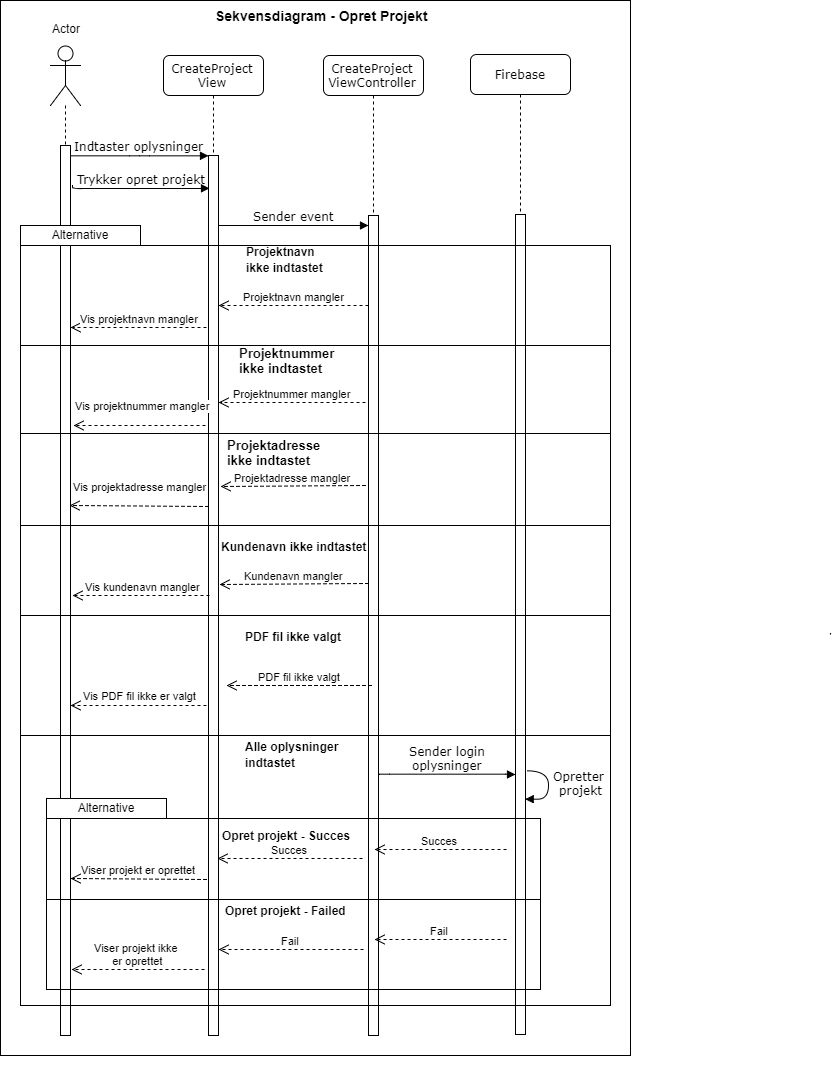
\includegraphics[height=18cm, width=15cm]{../ArkitekturDesign/Design/OpretProjekt/OpretProjektSekvensDiagram}
	\caption{Sekvensdiagram for 'Opret projekt' i Rambøll Tilsyn.}
	\label{fig:OpretProjektSekvens}
\end{figure}

\clearpage

På Figur \ref{fig:VaelgPDF} ses sekvensdiagrammet for 'Vælg PDF' i 'Opret Projekt' i Rambøll Tilsyn.
\begin{figure}[H] % (alternativt [H])
	\centering
	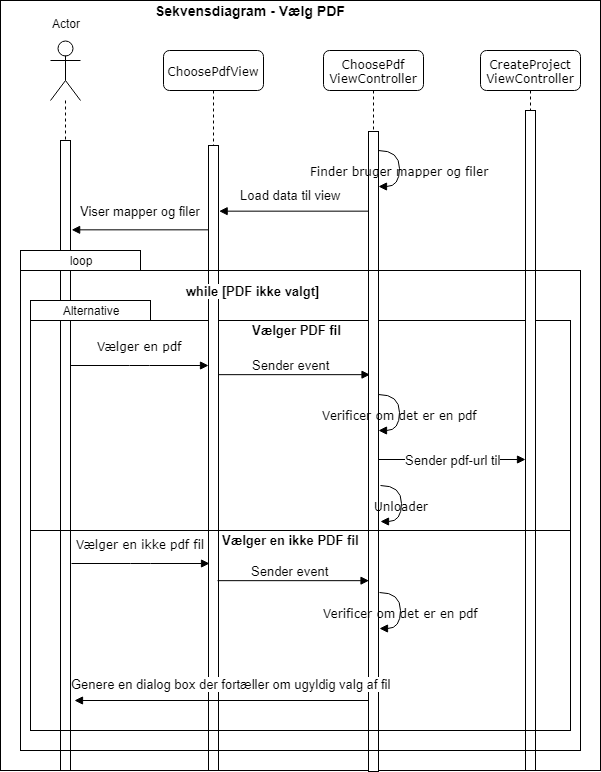
\includegraphics[height=15cm, width=12cm]{../ArkitekturDesign/Design/OpretProjekt/VaelgPdfDiagram}
	\caption{Sekvensdiagram for 'Vælg PDF' i 'Opret Projekt' i Rambøll Tilsyn.}
	\label{fig:VaelgPDF}
\end{figure}

\clearpage

\subsubsection{Grafisk brugergrænseflade}
I 'Opret  Projekt' viewet er der lavet felter til alle de informatior, som skal tastes ind om et nyt projekt. Se Figur \ref{fig:OpretProjektView}
\begin{figure}[H] % (alternativt [H])
	\centering
	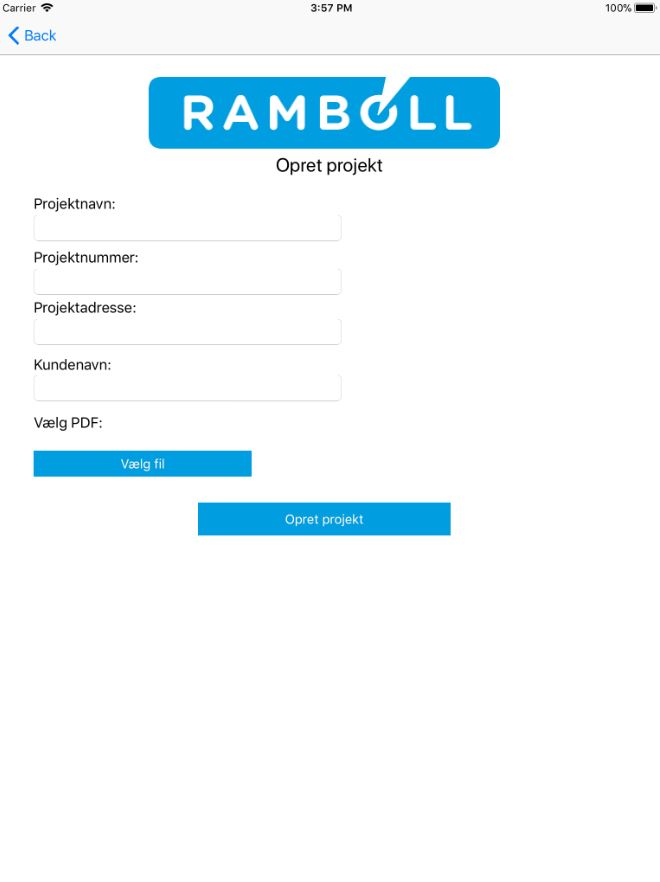
\includegraphics[height=12cm, width=10cm]{../ArkitekturDesign/Design/OpretProjekt/OpretProjektView}
	\caption{'Opret projekt' viewet som det er implementeret i Rambøll Tilsyn.}
	\label{fig:OpretProjektView}
\end{figure}

\subsubsection{Implementering}
Denne funktionalitet er ikke implementeret.

\clearpage